%! TEX root = ../main.tex
\chapter{Methodology}
\label{ch:methodology}

This chapter details the structural design, kinematic modeling, sensor integration, state estimation, and natural language dispatch architecture of the developed Autonomous Mobile Robot (AMR). The platform is engineered around an onboard Raspberry Pi~5 compute platform executing an integrated Python control stack, pairing omnidirectional Mecanum locomotion with visual SLAM, inertial sensing, sonar ranging, and LLM-assisted goal interpretation.

\section{System Architecture and Mechanical Design}
The AMR is constructed using a modular, dual-tier chassis configuration designed to physically isolate low-level electro-mechanical actuation and compute hardware from high-level perception and sensing instrumentation.

\subsection{Physical Chassis Configuration}
As shown in Fig.~\ref{fig:bot_view}, the platform comprises a rigid lower base plate and an elevated upper deck separated by cylindrical structural standoffs. 
\begin{itemize}
    \item \textbf{Lower Deck and Interior Bay:} Houses the primary compute platform (Raspberry Pi~5 single-board computer), drive actuators, motor drivers, battery power distribution, and system wiring harnesses.
    \item \textbf{Upper Deck:} Dedicated exclusively to the sensing and perception instrumentation, hosting the MPU-6050 6-axis Inertial Measurement Unit (IMU), the front ultrasonic distance sensor, and the elevated dual-camera mounting bridge.
    \item \textbf{Sensor Array Placement:} The front of the upper deck incorporates a dedicated vertical bracket securing the dual-transducer ultrasonic sonar sensor for forward distance ranging. The elevated top bridge supports the primary and secondary camera modules routed via dedicated CSI ribbon cables, alongside the surface-mounted MPU-6050 IMU.
    \item \textbf{Drive System:} Locomotion is achieved using four independently driven Mecanum wheels featuring angled peripheral rollers, providing full 3-DOF omnidirectional mobility in planar environments.
\end{itemize}

\begin{figure}[htbp]
    \centering
    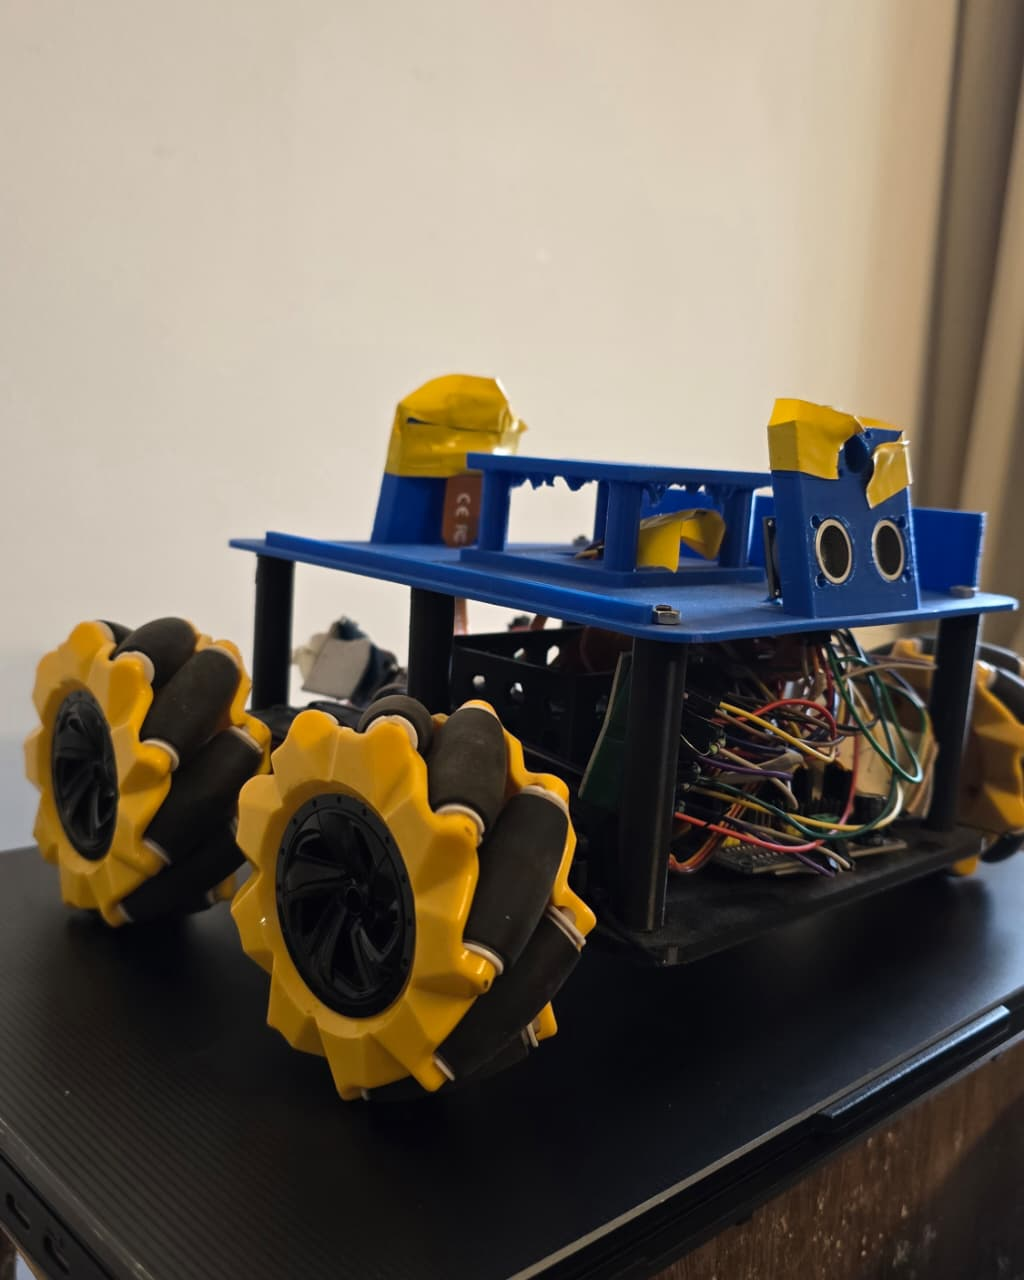
\includegraphics[width=0.62\textwidth]{Figures/Bot_view.jpeg}
    \caption{Assembled omnidirectional AMR prototype featuring the dual-deck chassis, four-wheel Mecanum drive train, front ultrasonic sensor bracket, upper sensing deck, and integrated electronics bay.}
    \label{fig:bot_view}
\end{figure}

\subsection{Hardware and Compute Interfacing}
The robot's computation and sensing stack comprises the following primary components:
\begin{enumerate}
    \item \textbf{Onboard Compute:} Raspberry Pi~5 (housed in the lower bay) executing a dedicated Python virtual environment (\texttt{robot\_env}) hosting low-level actuation scripts, sensory acquisition nodes, and SLAM pipelines.
    \item \textbf{Inertial Sensing:} An MPU-6050 6-axis sensor mounted on the upper deck and interfaced via I2C, acquiring 3-axis linear acceleration and 3-axis angular velocity data alongside onboard die temperature.
    \item \textbf{Ultrasonic Ranging:} A front-facing sonar module on the upper deck providing direct time-of-flight distance measurements for obstacle proximity alerts and reactive collision avoidance.
    \item \textbf{Dual-Camera Vision System:} A synchronized dual-camera setup positioned on the upper elevated bridge consisting of a primary forward-facing camera (\texttt{Cam~0}) and a secondary/stereo camera (\texttt{Cam~1}) for feature-based Visual SLAM and perception.
    \item \textbf{Power Monitoring:} An onboard voltage sensing divider continuously sampling battery supply voltage ($V_{\text{bat}}$) to track discharge characteristics during operation.
\end{enumerate}

\section{Omnidirectional Kinematic Modeling}
Unlike conventional differential drive architectures that are non-holonomic, the four-wheel Mecanum drive platform provides holonomic mobility. The robot can achieve independent linear translation along the longitudinal axis ($v_x$), lateral translation ($v_y$), and yaw rotational velocity ($\omega_z$) simultaneously without changing heading.

\subsection{Forward and Inverse Kinematics}
Let $r$ denote the radius of the Mecanum wheels, $l_x$ represent the longitudinal distance from the robot's center of mass to the wheel axes, and $l_y$ denote the lateral distance from the center of mass to the wheel centers. The inverse kinematic model maps desired body velocities $\mathbf{V} = [v_x, v_y, \omega_z]^T$ to the individual angular velocities of the four wheels $(\omega_1, \omega_2, \omega_3, \omega_4)$~\citep{siegwart2011introduction}:

\begin{equation}
\begin{bmatrix}
\omega_1 \\
\omega_2 \\
\omega_3 \\
\omega_4
\end{bmatrix}
= \frac{1}{r}
\begin{bmatrix}
1 & -1 & -(l_x + l_y) \\
1 &  1 &  (l_x + l_y) \\
1 &  1 & -(l_x + l_y) \\
1 & -1 &  (l_x + l_y)
\end{bmatrix}
\begin{bmatrix}
v_x \\
v_y \\
\omega_z
\end{bmatrix}
\label{eq:mecanum_kinematics}
\end{equation}

where $\omega_1$, $\omega_2$, $\omega_3$, and $\omega_4$ denote the angular velocities of the Front-Left, Front-Right, Rear-Left, and Rear-Right wheels, respectively.

By modulating individual motor directions and PWM duty cycles based on Eq.~(\ref{eq:mecanum_kinematics}), the platform executes six primary motion primitives: forward/backward translation, lateral strafing left/right, and in-place axial rotation.

\section{Low-Level Control, Calibration, and Teleoperation}
Low-level motion control and sensor interfacing are handled via dedicated Python modules within the onboard repository (\texttt{w\_move.py}, \texttt{move.py}, and \texttt{mpu6050.py}).

\subsection{Inertial Sensor Calibration and Teleoperation}
To mitigate sensor bias and temperature drift, an integrated MPU-6050 telemetry and teleoperation routine was developed. The script samples the accelerometer ($\text{m/s}^2$) and gyroscope ($\text{deg/s}$) across all three spatial axes while exposing a low-latency keyboard teleoperation matrix for manual system checkout.

\begin{figure}[htbp]
    \centering
    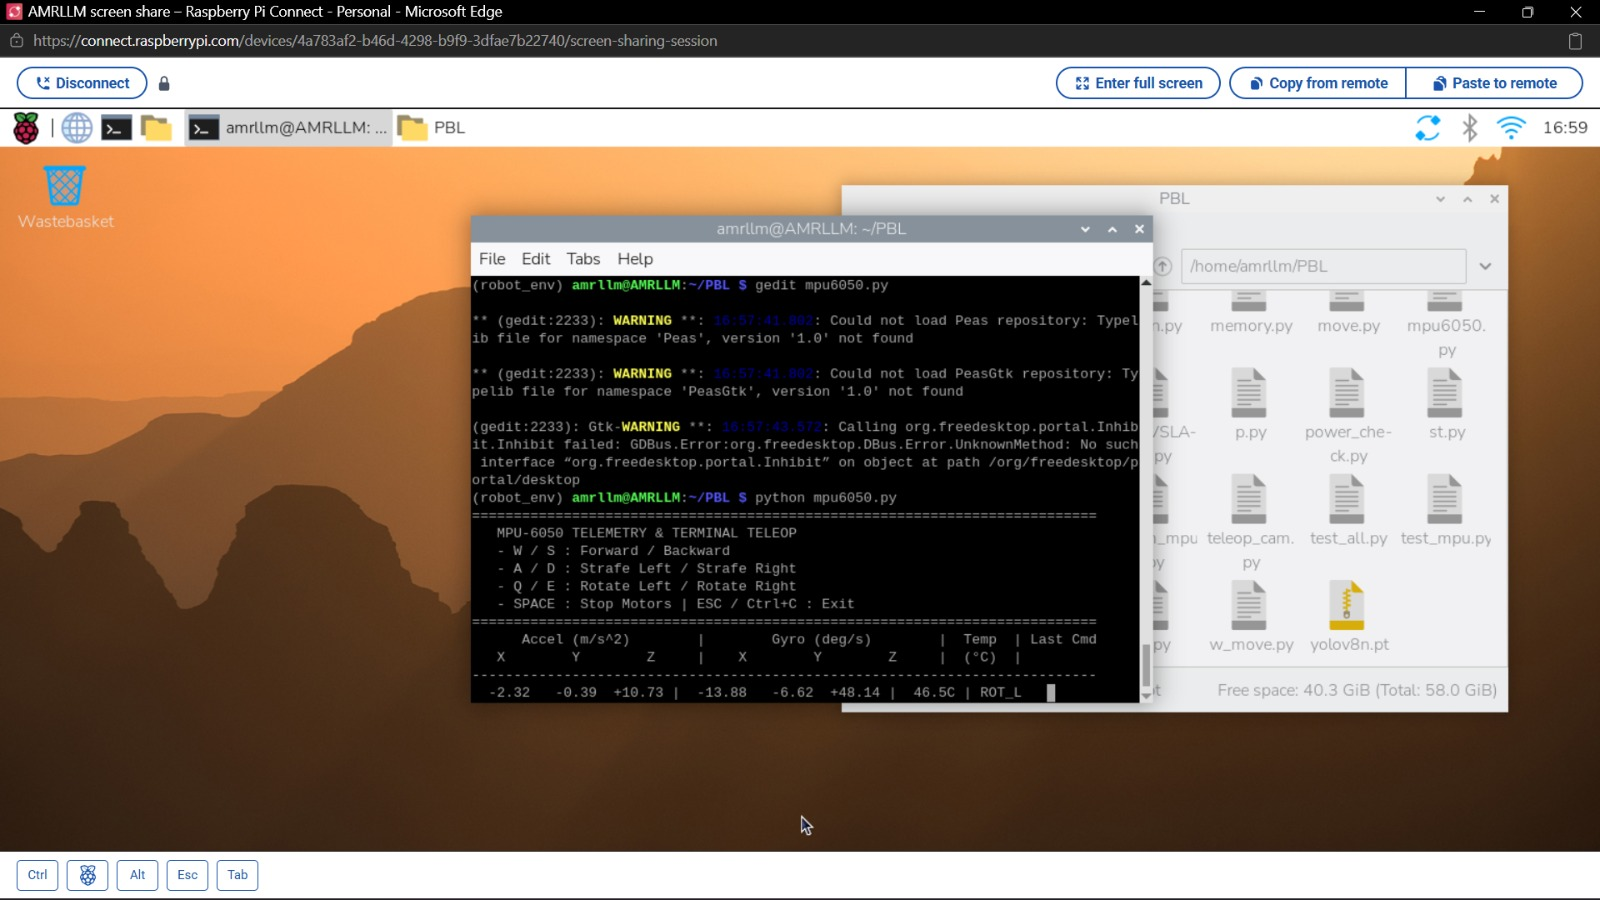
\includegraphics[width=0.85\textwidth]{Figures/GYRO_Callibration.jpeg}
    \caption{Real-time MPU-6050 IMU telemetry and terminal teleoperation interface running on the Raspberry Pi~5, displaying 3-axis acceleration, angular velocities, sensor temperature, and active motion command states.}
    \label{fig:gyro_calibration}
\end{figure}

As illustrated in Fig.~\ref{fig:gyro_calibration}, the teleoperation routine maps standardized control inputs:
\begin{itemize}
    \item \textbf{W / S:} Forward and backward longitudinal translation.
    \item \textbf{A / D:} Lateral strafe left and strafe right commands.
    \item \textbf{Q / E:} Counter-clockwise and clockwise rotational yaw commands.
    \item \textbf{Spacebar / Esc:} Instantaneous motor halt and routine termination.
\end{itemize}
The routine prints live inertial vectors, die temperature ($46.5^\circ\text{C}$), and the active actuation state (e.g., \texttt{ROT\_L}), ensuring motor command integrity and sensor health prior to autonomous routines.

\section{Visual SLAM and State Estimation}
Autonomous navigation without physical track constraints requires concurrent environmental mapping and ego-motion estimation~\citep{thrun2005probabilistic}. The platform deploys feature-based Visual SLAM (V-SLAM) leveraging the ORB-SLAM2 framework.

\subsection{ORB Feature Tracking and Map Point Generation}
The vision pipeline ingests real-time video frames from the primary camera (\texttt{Cam~0}) and stereo secondary camera (\texttt{Cam~1}) mounted on the upper deck. ORB (Oriented FAST and Rotated BRIEF) feature points are extracted across successive image frames. By computing FAST corners with orientation descriptors and matching corresponding BRIEF descriptors across baseline frames, the system computes:
\begin{enumerate}
    \item \textbf{Feature Landmark Triangulation:} Three-dimensional spatial coordinates for persistent visual landmarks across the environment.
    \item \textbf{Ego-Motion Estimation:} Motion transformations $[R | t]$ between consecutive frames, determining robot translation and yaw angle.
    \item \textbf{Bundle Adjustment:} Continuous optimization minimizing reprojection errors between observed feature locations and predicted landmark projections.
\end{enumerate}

\subsection{Real-Time Environmental Tracking and Telemetry Integration}
The V-SLAM pipeline executes concurrently on the Raspberry Pi~5, continuously estimating spatial poses ($X, Y, \text{Yaw}$), updating 3D landmark clouds, and acquiring forward ultrasonic range distances alongside battery state of charge. The full visualizer interface and experimental trajectory outcomes are presented and evaluated in Chapter~\ref{ch:results_and_discussion}.

\section{Vision-Based Object Detection}
In addition to geometric feature tracking, semantic environmental understanding is provided through an integrated YOLOv8 object detection model (\texttt{yolov8n.pt}) deployed within the onboard environment. By passing frames from the primary camera through the compact YOLOv8 network, the system detects and classifies key operational objects and obstacles in real time, supplying semantic labels to the spatial navigation memory.

\section{Natural Language Command Parsing Pipeline}
To bridge human operational commands with the autonomous navigation stack, the AMR incorporates an NLP/LLM interpretation engine~\citep{brown2020language, openai2024gpt}.

\subsection{Prompt Formatting and Entity Extraction}
Unstructured plain-English instructions entered by human operators (e.g., \textit{``Move forward to the inspection station''} or \textit{``Navigate to desk one''}) are processed via a structured prompt completion pipeline. The language model extracts two core parameters:
\begin{itemize}
    \item \textbf{Intent Classification:} Categorizing whether the command denotes a navigation task, a stop request, or a status query.
    \item \textbf{Target Entity Identification:} Isolating the specific semantic destination or landmark reference from conversational phrasing.
\end{itemize}

\subsection{Spatial Grounding via Topological Memory}
The parsed destination entity is cross-referenced against the local coordinate repository (\texttt{memory.py}). This database associates recognized semantic labels with calibrated Cartesian target poses $(x^*, y^*, \theta^*)$ previously registered within the SLAM map coordinate frame. Once matched, the target coordinates are passed directly to the onboard motion controller, which computes the required Mecanum velocity vectors to drive the robot to the goal pose while monitoring sonar thresholds for path clearance.

\section{Real-Time Operational Monitoring}
System health, pose tracking, and diagnostic telemetry are aggregated locally on the Raspberry Pi~5. The operational visualizer presents live metrics—including planar trajectories, active landmark clouds, battery discharge voltage, sonar range measurements, and motion states—directly within the desktop environment. This unified interface provides operators with complete supervisory visibility into both algorithmic SLAM execution and low-level electromechanical performance without loading the real-time control loop.